\chapter{Porting Tang}\label{porting-tang}

After successfull cross-compilation of jose we have all the dependencies "ready" and packaged except the systemd.
systemd is only one of the many implementations (inetd, launchd, ucspi-tcp, xinetd) of a super-server providing socket activation.



\section{Socket activation}\label{socket_activation}

Socket activation is a technology provided by a super-server (also called a service dispatcher daemon).
A super-server starts other servers when needed as well, normally with access to them checked by a TCP wrapper.
It uses very few resources when in idle state.

A service designed for the socket activation would behave as bare CLI application with input read from stdin (standard input) and output written to stdout (standard output).
Tang is exactly this kind of an application and because of that we need to configure socket activation\cite{super_server}.



\subsection{xinetd}
xinetd listens for incoming requests over a network and launches the appropriate service for that request.
Requests are made using port numbers as identifiers and xinetd usually launches another daemon to handle the request.
This is reflected on Figure \ref{fig_xinetd} xinetd socket activation below.
\begin{figure}[h]
    \centering
    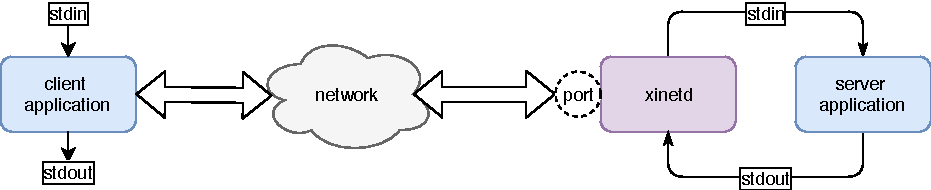
\includegraphics[scale=0.9]{figures/xinetd.pdf}
    \caption{xinetd socket activation}
    \label{fig_xinetd}
\end{figure}
xinetd features access control mechanisms such as TCP Wrapper ACLs (access control lists), extensive logging capabilities, and the ability to make services available based on time.
It can place limits on the number of servers that the system can spawn.
xinetd is listening on behalf of the services.
Whenever a connection would come in an instance of the respective service will be spawned with using stdin and stdout of the service application\cite{xinetd}.



\section{Package the Tang}
Similarly to José we need to create a new package for OpenWrt.
The Tang project is owned by same owner on GitHub as José.
We sould visit the project releases page\footnote{https://github.com/latchset/tang/releases/} and get the Tang version v6.
Then add following lines to the Makefile similarly as with José's Makefile:
\begin{lstlisting}[columns=fixed,basicstyle=\ttfamily\footnotesize,tabsize=4,backgroundcolor=\color{yellow!10}]
include $(TOPDIR)/rules.mk

PKG_NAME:=tang
PKG_VERSION:=6
PKG_RELEASE:=1

PKG_SOURCE:=$(PKG_NAME)-$(PKG_VERSION).tar.bz2
PKG_SOURCE_URL:=\
https://github.com/latchset/$(PKG_NAME)/releases/download/v$(PKG_VERSION)/

PKG_HASH:=1df78b48a52d2ca05656555cfe52bd4427c884f5a54a2c5e37a7b39da9e155e3


PKG_INSTALL:=1
PKG_BUILD_PARALLEL:=1

PKG_FIXUP:=autoreconf

include $(INCLUDE_DIR)/package.mk
\end{lstlisting}
Do not forget to add the package description which should have section dependencies filled.
The libhttp-parser dependency used for parsing HTTP requests.
José the library and tool for the Javascript Object Signing and Encryption.
xinetd is a runtime dependency, the actual build proccess of the Tang does not require its libraries but to have its socket activation available in runtime.
The bash dependency is there for a good reason.
The Tang's update and key generation executables are bash scripts.
\begin{lstlisting}[columns=fixed,basicstyle=\ttfamily\footnotesize,tabsize=4,backgroundcolor=\color{yellow!10}]
define Package/tang
  SECTION:=utils
  TITLE:=tang v$(PKG_VERSION) - daemon for binding data to the presence of a third party
  DEPENDS:=+libhttp-parser +xinetd +jose +bash
  URL:=https://github.com/latchset/tang
endef
\end{lstlisting}
Let us add a brief description to
\begin{lstlisting}[columns=fixed,basicstyle=\ttfamily\footnotesize,tabsize=4,backgroundcolor=\color{yellow!10}]
CFLAGS += -fhonour-copts
TARGET_CFLAGS += $(FPIC) -std=gnu99 -D_GNU_SOURCE
TARGET_LDFLAGS += -Wl,-rpath-link=$(1)/usr/lib

define Package/tang/description
	Tang is a small daemon for binding data to the presence of a third party.
endef
\end{lstlisting}


\begin{lstlisting}[columns=fixed,basicstyle=\ttfamily\footnotesize,tabsize=4,backgroundcolor=\color{yellow!10}]
define Package/tang/install
	$(INSTALL_DIR)	$(1)/usr/libexec
	$(INSTALL_DIR)	$(1)/etc/xinetd.d/
	$(INSTALL_BIN)	$(PKG_INSTALL_DIR)/usr/lib/$(PKG_NAME)d*	$(1)/usr/libexec/
	$(INSTALL_BIN)	./files/tangdw	$(1)/usr/libexec/
	$(CP)			./files/tangdx	$(1)/etc/xinetd.d/
endef
\end{lstlisting}
And do not forget the last line which allows the actual "magic" to happen:
\begin{lstlisting}[columns=fixed,basicstyle=\ttfamily\footnotesize,tabsize=4,backgroundcolor=\color{yellow!10}]
$(eval $(call BuildPackage,$(PKG_NAME)))
\end{lstlisting}

After first run we will encounter the systemd dependency errror:
\begin{lstlisting}[columns=fixed,basicstyle=\ttfamily\footnotesize,tabsize=4,backgroundcolor=\color{yellow!10}]
configure: error: Package requirements (systemd) were not met:

No package 'systemd' found

Consider adjusting the PKG_CONFIG_PATH environment variable if you
installed software in a non-standard prefix.
\end{lstlisting}
We did not defined it for Makefile but the cross-compilation of the package will try to configure and compile downloaded sources.
Compiler will try to find the systemd dependency as it is defined in the "file" in Tang repository.
We shall remove this builtime dependency.

As we studied the autotools files Makefile.am and the configure.ac and removed the systemd related requirements and dependency we founf a definition to
Diffs can be found when following propper link on appendix \label{diffs} List of pull-request.

\todo{text and diff for makefile and configure}

After removal the build will be successfull and we have Tang package ready to be installed on our device.
We are avoiding troubles with using the libhttp-parser in version 2.8.0.
These self issued problems are described in following subsection \ref{http_parser_problems} Hurdles with http-parser.
The most important part after successfull build would be to configure it right way.



\subsection{Hurdles with http-parser}\label{http_parser_problems}

without upstream patch not working tang \todo{text}
\newpage



\subsection{Mysterious José}

does makefiles support shell {a,b} thing???
\newpage
